%Paper model
Although often disregarded in many experimental and theoretical studies, neural sequences are key elements of brain activity which, in many cases, have a direct relationship to behavior \parencite{hahnloser_ultra-sparse_2002,venaille_synchronization_2005,hb10,buzsaki_space_2018,rabinovich_discrete_2018,paton_neural_2018,elices_robust_2019}.
%This neural sequences have been observed experimental and theoretically, and are considered to be the ones carrying information in the neural system, playing an important role in the function these systems generate. 
The study of neural sequences involves the assessment of time references, time intervals and the associated temporal structure of individual neurons, groups of neurons or large neural ensembles, which typically hinder their characterization due to experimental limitations. In this context, Central Pattern Generators (CPGs) are adequate neural circuits to study the generation and coordination of neural sequences. 
%Hence, when studying neural activity it is not only important the response a single cell might produce (measured in form of ISI analysis, return maps, etc.) but the interaction it has in a whole circuit. It is due to the interaction between different cells and the effect of the synapses they are affected by, that some function in a living element is generated. Indeed, many motor rhythmic activity have their origin in closed cell circuits. This is the case of Central Pattern Generators (CPGs).
CPGs are neural structures capable of generating rhythmic activity that involves robust motor sequences in a highly autonomous manner \parencite{hartline_mottor_1976,selverston_reliable_2000,marder_central_2001}. This kind of circuits are found in many different organisms including humans \parencite{dimitrijevic_evidence_1998,pavlidis_neonatal_2016, arichi_localization_2017}. CPG neurons have rich intrinsic dynamics and their connections form non-open circuit topologies in which all members of the circuit receive information from at least another member in the ensemble \cite{selverston_reliable_2000,huerta_topology_2001}. This favors rhythm coordination through closed-loop computation and endows CPGs with the ability to produce robust yet flexible rhythms where intervals building the sequences can be adapted in different behavioral contexts \parencite{elices_robust_2019}. %These intervals building the sequences cycle-by-clycle, are defined as different temporal events in each neuron, such as burst duration. 
In Fig. \ref{fig:sequences_in_cpgs} there is an example of the robust sequential generation of bursts in a CPG. 

\begin{figure}[htb]
	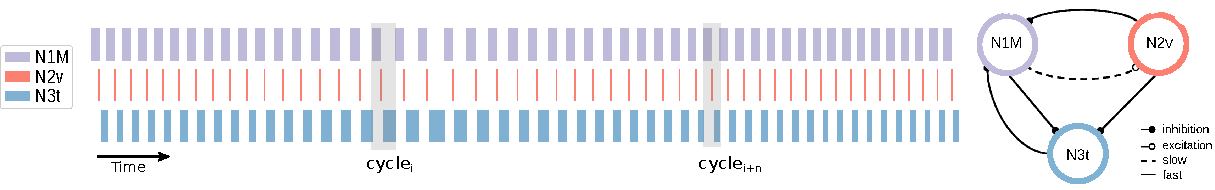
\includegraphics[width=\textwidth]{img/invariants/variability/sequences_in_cpgs.pdf}
	\caption{Example of robust sequential bursting dynamics in CPGs. Representation of burst duration in 3 neurons in a CPG model, the sequential activation of the three neurons conform cycles (transparent grey boxes in the sequence). The connections between the three neurons are represented in the diagram on the right side of the panel.}
	\label{fig:sequences_in_cpgs}
	
\end{figure}

The sequence of intervals underlying CPG rhythms present variability in the duration of each cell activation/inactivation, which has been identified in different nervous systems, e.g. see \cite{reyes_artificial_2008,elliott_temporal_1991,martinez_short-term_2019}. Consequently to the study of variability in cycle-by-cycle sequences, we have recently found sequential dynamical invariants in the form of robust linear relationships between specific sequence intervals and the period in the pyloric CPG of shore crabs (\textit{Carcinus maenas}) \cite{elices_robust_2019}. Dynamical invariants represent constraints of particular sequence intervals in relation to different intervals in the same cycle as the instantaneous duration of the period and build rules for the overall flexibility of the rhythm. It is important to note that not all intervals composing the sequence display such constraints. The presence of invariants in the crustacean pyloric CPG are observed in all control conditions as well as in experiments under the effect of ethanol, which induces irregular rhythms \cite{elices_robust_2019}. 

%\red{Moreover, different experimental cases are described in this study, including recordings with ethanol and PTX application. The invariants were found to be present even under those circumstances which alter the neurons activity and their variability}.

%settle an evidence in the strong relation between the sequential activation and the period duration, highlighting the importance of the temporal variability which is always present in the same intervals.

While the existence of phase maintenance and linear relationships between rhythm intervals and the period have been discussed before in convenient animal models, e.g. \cite{grillner_generation_1976,hooper_phase_1997,vavoulis_dynamic_2007}, detailed characterization of cycle-by-cycle variability to understand the existence of these relationships and the corresponding analysis of the universality of robust dynamical invariants are pending.

During this chapter we will characterized the sequence interval variability in a model of the \textit{L. stagnalis} feeding CPG inducing variability with a ramp current injection, we will also address the issue of variability in models to study this kind of phenomena, and explore and discuss the presence of sequential dynamical invariants in living intracellular recordings as well as their possible functional role by inducing the activity from different methods but also from a practical approach in robotics. 

%In particular, a thorough analysis of interval variability in CPG models and their use in understanding the generation of dynamical invariants within specific time intervals have not been addressed. The main difficulty to study the functional balance between flexibility and robustness in sequences generated by theoretical models is the lack of variability both in the intrinsic and network dynamics. In this paper, we report the characterization of sequence interval variability in a model of the \textit{Lymnaea} feeding CPG.  By using ramp current injection protocols, it is possible to induce variability in the collective activity of the neurons of this CPG model. This enables the study of the evoked variability of the intervals conforming each cycle following the same interval definitions from \cite{elices_robust_2019}, as well as the conceivable presence of dynamical invariants, which we address here. 

